\section{Project management}
\label{section:project_management}

We will discuss in this section everything concerning the management of the project: \textit{scope}, \textit{schedule} and \textit{budget}. However, we must stress that this classical approach of management analysis is not really suited for our needs. Instead, a more \textit{Agile}\footnote{Agile software development is based on the \textit{Agile manifesto}~\cite{website:AgileManifesto}.} methodology will be applied. We cover this on the Methodology section, but there is an important conceptual change to be taken into account: the different driving force of the project. Whereas in classical project management the scope-schedule-budget triad is what must be controlled, in an Agile project management approach it is \textit{value}. Indeed, \textit{quality} must be ensured so maximum value is delivered to the project's stakeholders, thus being scope, cost and schedule constraints to these primary goals.

\begin{figure}[h]
	\centering
	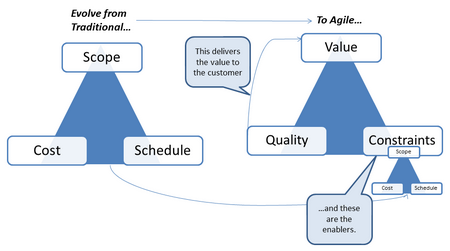
\includegraphics[width=0.7\linewidth]{figures/agiletriangle-1.png}
	\caption{Traditional to Agile project management evolution. Source:~\cite{website:AgileTriangle}}
	\label{fig:agile-pm}
\end{figure}

\subsection{Scope}
\label{section:scope}

One of the first things to do, when beginning any project is delimiting its scope, this is, deciding \textit{what} will be done and \textit{how}, in terms of resources and methodology, for example.

\subsubsection{Requirement analysis}

We already stated in section~\ref{section:introductionNutshell} what the main goal of this project is. A more detailed list of the project's requirements is the following one:

\begin{itemize}
	\item \textbf{Functional requirements:} 
	\begin{enumerate}
		\item Implement privacy preserving stream mining \textit{filters}\footnote{Within the MOA context, \textit{filters} are procedures applied to data prior to their analysis using machine learning algorithms.} for the MOA stream mining framework. The suggested algorithms to be implemented are:
		\begin{enumerate}
			\item Noise addition~\cite[p.~54]{book:StatisticalDisclosureControl}
			\item Multiplicative noise~\cite[p.~57]{book:StatisticalDisclosureControl}
			\item Microaggregation~\cite[p.~60]{book:StatisticalDisclosureControl}
			\item Rank shuffling~\cite[p.~73]{book:StatisticalDisclosureControl}
			\item Differential privacy~\cite{Dwork06differentialprivacy}
		\end{enumerate}
	\end{enumerate}
	
	\item \textbf{Non-functional requirements:}
	\begin{enumerate}
		\item \textbf{Correctness:} privacy protection is at stake in this project, so algorithms must be implemented correctly, from the theoretical point of view, in order to not ease information disclosure when they are used.
		\item \textbf{Efficiency:} given that no data mining process can scale well if its algorithms are slow, effort will be put in making them the most efficient we can.
		\item \textbf{Test coverage:} measures and tests will be performed to assess the quality of the developed software, as well as its scalability and performance, which is paramount in this project’s context.
		\item \textbf{Documentation:} MOA is an \textit{open source} data mining framework, which means that its community can assess how is it built and how to improve it. One of the benefits of the open source development model is that software can be safer, more robust and efficient, by receiving contributions from different developers. If people are to continue improving the work done, it has to be well documented.
	\end{enumerate}
\end{itemize}

\subsubsection{Scope risks analysis}

The methodology approach used in this project will be based on Agile principles. This involves several decisions on how to manage the project and its requirements.\\

In this particular project, if we are to examine the classic constraints that we talked about at the beginning of this section, we do know that the schedule is fixed (perhaps not the planning, but the final milestone) and this forces us to let the scope opened. This is, we will implement as much features as we can, assessing their quality, but no feature list will be fixed from the beginning of the project.\\

Because we will be working on the basis of an \textit{open scope}, deviations in this field are likely to happen. These, however, will not pose to be a project failure in any case, because it has been agreed to be developed this way.

\subsubsection{Methodology}

Agile methods will be applied throughout the development phase of this project. Some of the key concepts and practices in this respect are:

\begin{itemize}
	\item Short to mid range development \textbf{sprints} (phases), in order to keep track of the project’s evolution and to be able to react to changes, unforeseen constraints or scope drifts.
	\item \textbf{Constant meetings} with the project’s stakeholders, in which the progress and deviations of the project will be assessed. Measures to alleviate them will be taken in these meetings.
	\item Use of \textbf{burndown charts} - graphical representations of work left to do versus time.
\end{itemize}

\subsection{Schedule}

\subsubsection{Overall duration}

Taking a general look at the project’s schedule, we can estimate it to have a total duration of about 5 months. Even though it was registered on July, 2014, the project did not begin until September, because August is the only month I can have holidays, due to job restrictions. Considering the next possible project’s lecture shifts, we believe that the one taking place in December is too close in time. Thus, the project will endure until January the 26th, 2015. This should give us time enough to develop the project and document it without too much pressure, which is key to fulfill one of the main established goals: high quality results.

\subsubsection{Schedule slack}

The project schedule we present herein does not fill up the total amount of time available - more than two weeks are left blank, with no assigned tasks. This is intended because of the following reasons:

\begin{itemize}
	\item The amount of time needed to develop the proposed algorithms is uncertain. It is hard to estimate the time it may take, because I have no previous knowledge on the area. Therefore, we opted for, in one hand, an \textit{open scope} approach, and, on the other, leaving a considerable time gap between the last planned task and the project’s final milestone: its defense. Being conservative, if the development of any proposed method is delayed, we still have some leeway to introduce schedule changes, without risking the project’s success.
	
	\item We have estimated the project’s report confection and the defense presentation rehearsals to be 35 and 7 days, respectively, but depending on how much development is finally carried out, it might not be time enough to write down the report. Extra time for doing it can be then borrowed from the schedule slack time.
	
\end{itemize}

\subsubsection{Schedule monitoring \& changes}

For the development phase of the project, the most suitable way to monitor the schedule we have found is applying an Agile approach to the process. We will work in one week long sprints, meeting every week to assess the quality of the solutions, the proper progress of the project and to plan what will be done during the following sprint.\\

Sprint planning meetings are where the main goals of the project will be sliced in small tasks, which can be tracked and implemented better, because they are not so complex. Thanks to this constant fine-grained planning process, schedule or scope deviations are detected earlier and can be managed efficiently, reacting before they affect deeper the overall success of the project. Given that no fixed features list is assigned to each sprint of the development phase, if the completion of either of those features is delayed, it can be made to span for some more time.\\

Within each of the development sprints, burn downcharts will be used to monitor the progress of the sprint. These charts are helpful in identifying patterns of work (sprint-end rushes, for example) and can help developers maintain a constant rate of finished features.\\

Besides burn down charts and sprint planning meetings, the use of velocity charts will also be helpful to increase the predictability of the following sprint plannings. The more predictable they are, the less deviations will occur and the schedule will be more likely to be fulfilled.

\subsubsection{Project phases}

The project is divided in 4 main phases, besides of the undertaking of the Project's Management module. Each phase has an estimated duration and a risk evaluation in terms of schedule deviation. The amount of hours is an approximated calculation from the number of days in each phase: 4 hours a day are estimated to be spent, because I am currently working part-time and also taking some subjects. A more detailed task granularity can be seen in the Gantt chart. Task dependencies are shown in the chart too. Those phases, chronologically ordered are:

\begin{enumerate}
	\item \textbf{Contextualization}: it is intended to perform a deeper bibliographic research and a study of the main subjects concerning the project, at the theory level - no practical skills or technological research will be done.
	\begin{itemize}
		\item \textbf{Duration estimation:} 11 days (44 hours).
		\item \textbf{Risk:} this phase has a medium to high risk of being delayed, due to lack of effective time (a wrong estimation), and also because more insight than planned might be needed, consuming more time.
	\end{itemize}
	
	\item \textbf{Environment setup}: during this phase, all necessary tools and material resources will be gathered and configured. The concrete developing workflow will be decided, too.
		\begin{itemize}
			\item \textbf{Duration estimation:} 8 days (32 hours).
			\item \textbf{Risk:} this phase has a low risk of being delayed, because the technology that is to be used is, a priori, well known to us.
		\end{itemize}
		
	\item \textbf{Development}: all of this project coding will be performed during this phase. As said before, a sprint methodology will be used during this phase, being one week each.
		\begin{itemize}
			\item \textbf{Duration estimation:} with an initial planning of 7 sprints, 49 days will be used (196 hours).
			\item \textbf{Risk:} there is a medium risk of this phase to be delayed. Even with the use of Agile methodologies, if a fundamental feature was needed and there was no more time left, another sprint (or at most a couple of them) could be introduced, to finish the remaining tasks.
		\end{itemize}
		
	\item \textbf{Documentation}: the project’s report will be written after the development phase, along with any deployment documentation that was required and the final presentation, which will also be rehearsed then.
		\begin{itemize}
			\item \textbf{Duration estimation:} 42 days (168 hours).
			\item \textbf{Risk:} this phase has a medium risk of being delayed too. Reviews of the report will be made and writing in English might take up more time than expected.
		\end{itemize}
	
\end{enumerate}

\subsubsection{Detailed schedule: Gantt chart}

The following chart was generated with the Project management free software package, available online on the Ubuntu 12.04 Software Center. Please note that there is no way the chart could fit in a single page (not even if it was landscape).

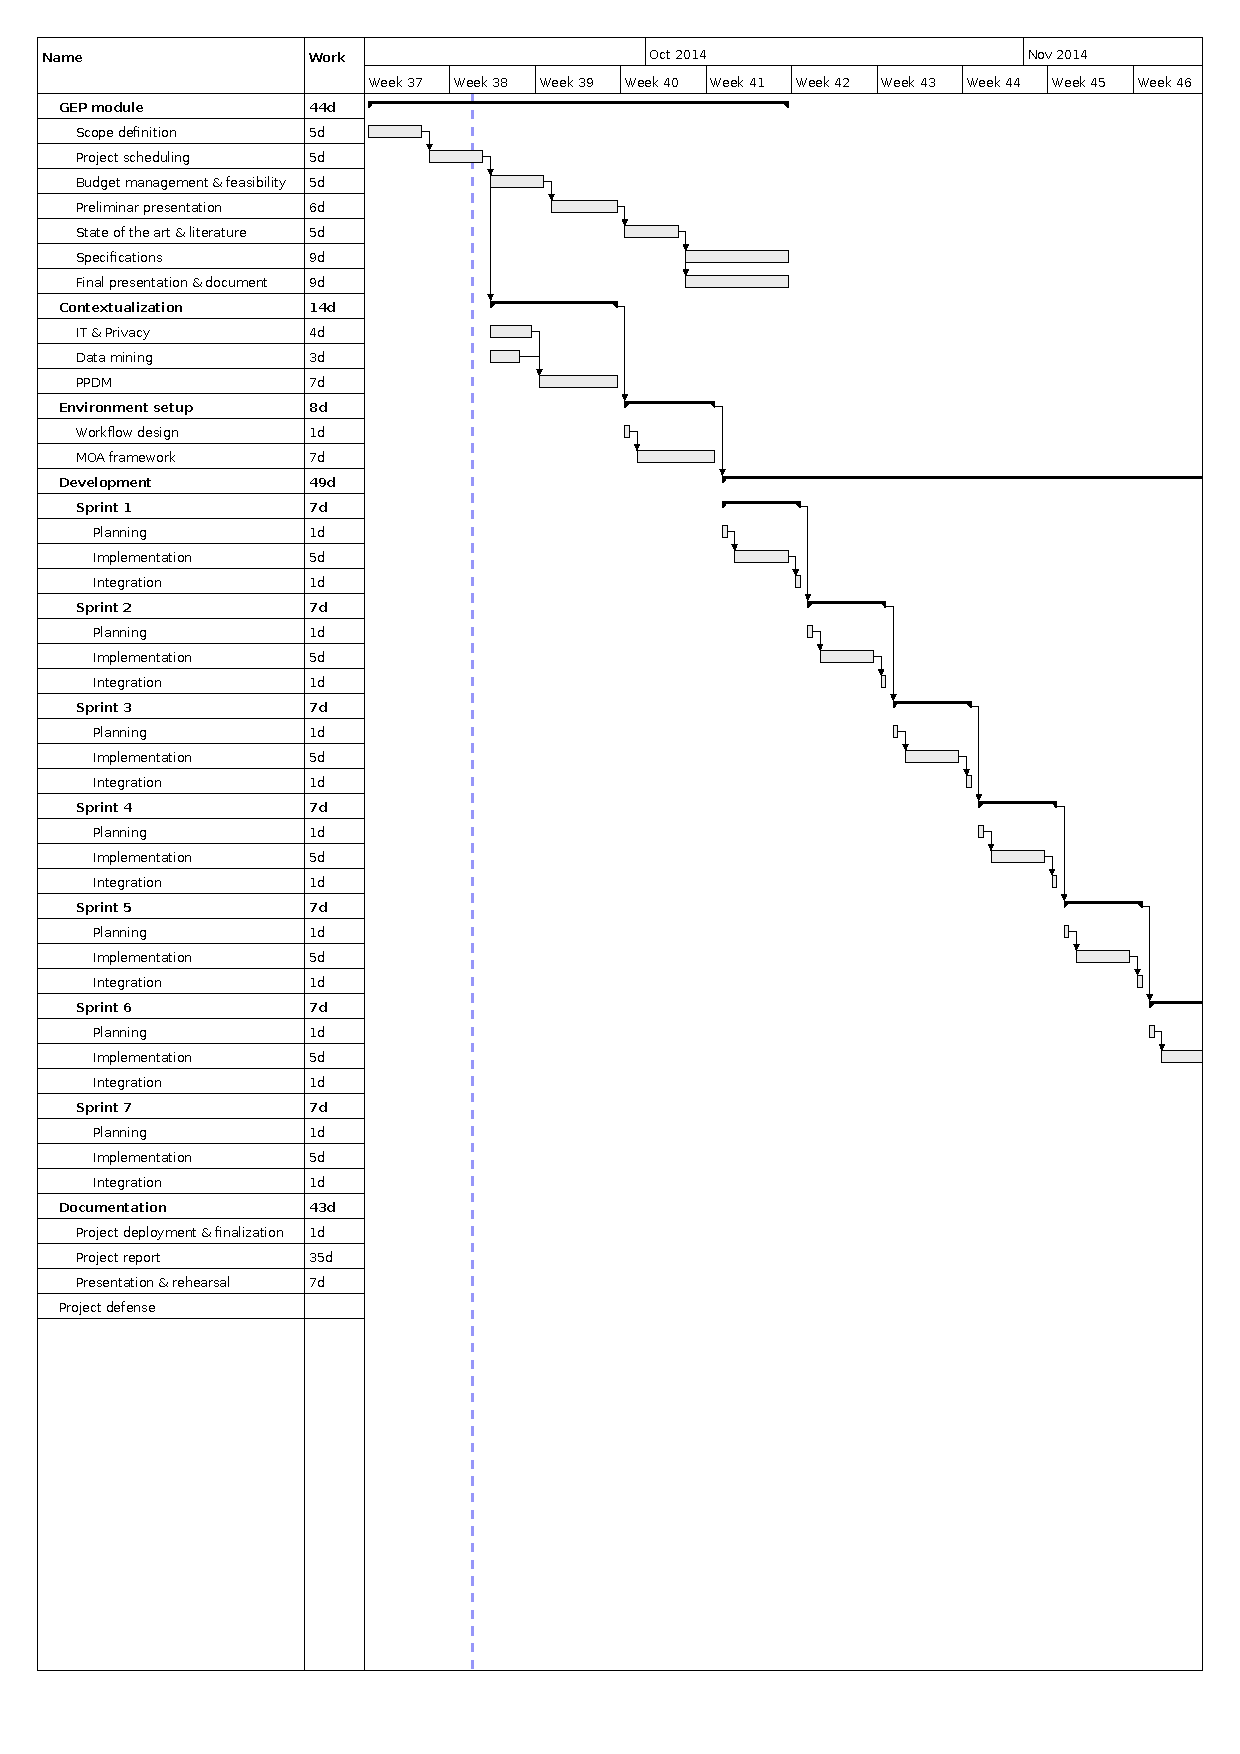
\includepdf[pages={1,2}]{figures/gantt-chart.pdf}

\subsection{Resources}

Resources consumed in this project only fall in one of the following categories: \textit{human resources}, \textit{hardware}, \textit{software} and \textit{other expenses}. For a detailed description of what will be needed in the project, please see the following section, on Budget management. It is important to keep in mind that \textit{all} resources will be consumed equally througout the entire project duration.

\subsection{Budget}

The project’s budget is entirely based on an estimation of human, hardware and software resources costs. No real income is perceived, besides the salary of the project’s supervisor, who is a tenure-track lecturer at the Barcelona School of Informatics, and an associate researcher at the Barcelona Supercomputing Center. No third parties are involved in the project - no companies or organizations are providing any funds. Moreover, even though the work is to be integrated into the MOA framework, it is indeed an open-source project, to which we will be contributing, meaning contributions are expected from any kind of source, be it funded or not.\\

All other associated costs are \textit{externalized}, either by people involved in the project or by the university, where the development of the project will be held.

\subsubsection{Budget estimation}

The total cost of the project is derived from the sum of the following items:

\begin{itemize}
	\item \textbf{Human resources:} (summarized in table~\ref{table:human-resources})\\
	All expenses included here are related to people’s salaries. Only one developer will be working on this project, but a number of hours involving supervision tasks is also imputed to the project’s supervisor, so its corresponding cost is added too. Taxes are included in all of the following items. The price is also an estimation: on the developer’s side, it is based on a salaries comparison webpage (\textit{Glassdoor}~\cite{website:glassdoor})\footnote{As of date 12th October, 2014, the average salary for a software engineer in Barcelona is 32000€ per year (including taxes). Considering 12 monthly instalments and an average of 160 hours per month, this yields a total of 16.66€ per hour.}; on the supervisor side, the price is based on his own estimation.
	\begin{itemize}
		\item \textit{Developer:} an average of 20 hours a week are estimated, spanning for about 21 weeks, summing up a total of 420 hours.
		\item \textit{Supervisor:}
		\begin{itemize}
			\item Project’s take off: 8 hours, between meetings and initial planning.
			\item Sprints: 8 hours each sprint, taking into account both face to face meetings and other supervising tasks. There are 7 sprints scheduled so far, making a total of 56 hours.
			\item Documentation: during the project’s final stage, an estimation of 20 hours is taken from the corresponding supervision of the project’s report.
		\end{itemize}
	\end{itemize}
	\begin{table}[h]
	\centering
	\begin{tabular}{lllr}
	\hline
	\textbf{Role} & \textbf{Price (per hour)} & \textbf{Working  hours} & \multicolumn{1}{l}{\textbf{Total}} \\ \hline
	Supervisor & \multicolumn{1}{r}{35€} & \multicolumn{1}{r}{84} & 2940€ \\
	Developer & \multicolumn{1}{r}{16.66€} & \multicolumn{1}{r}{420} & 6997.2€ \\ \hline
	 &  & \multicolumn{1}{r}{\textbf{Total}} & \textbf{9937.2€}
	\end{tabular}
	\caption{Human resources associated costs. All taxes are included in the Price per hour column.}
	\label{table:human-resources}
	\end{table}
	
	\item \textbf{Hardware:} (summarized in table~\ref{table:hardware-resources})\\
	All hardware needed resources are shown in the corresponding table. Their cost is calculated by estimating its amortization, spanned over 5 years (it is a personal laptop). To calculate its amortized cost per hour, we will take into account that this equipment is used throughout the course too, and estimating that 2500 hours of work are carried each year.
	\begin{table}[h]
	\centering
	\begin{tabular}{l r r r r r}
	\hline
	\textbf{Product} & \multicolumn{1}{l}{\textbf{Price}} & \multicolumn{1}{l}{\textbf{Units}} & \multicolumn{1}{p{3cm}}{\textbf{Amortized price per hour}} & \multicolumn{1}{l}{\textbf{Work time (hours)}} & \multicolumn{1}{l}{\textbf{Total}} \\ \hline
	Asus k53sv & 650€ & 1 & 0.052€ & 420 & 21.84€ \\ \hline
	 &  &  &  & \textbf{Total} & \textbf{21.84€}
	\end{tabular}
	\caption{Hardware amortization costs. All taxes included.}
	\label{table:hardware-resources}
	\end{table}
	
	\item \textbf{Software:}\\
	All software needed to undertake this project is free and, most of it, is open sourced. Despite this, we will include a list of it here, to show what will be used at a finer grain.
	\begin{itemize}
		\item \textit{Ubuntu 12.04}: operating system. Available at: \url{http://www.ubuntu.com/download}.
		\item \textit{Trello}: online task management tool. Available at: \url{https://trello.com/}.
		\item \textit{Google Drive}: online, collaborative office software suit, used to create burndown charts (spreadsheets). Available at: \url{https://drive.google.com}.
		\item \textit{Java SDK}: Java language Software Development Kit. Available at: \url{http://openjdk.java.net}.
		\item \textit{Eclipse IDE}: integrated development environment package. Available at: \url{https://www.eclipse.org/home/index.php}.
		\item \textit{Git}: source version control system. Available at: \url{http://git-scm.com/}. Remote code repositories will be hosted at GitHub (\url{https://github.com}) for free.
		\item \textit{MOA}: Massive Online Analysis, a stream mining framework. Available at: \url{http://moa.cms.waikato.ac.nz}.
		\item \LaTeX: document preparation system. Available at: \url{http://www.latex-project.org}.
	\end{itemize}
	
	\item \textbf{Other expenses:}\\
	All expenses not covered in the previous sections are detailed in table~\ref{table:other-resources}.
	\begin{table}[h]
	\centering
	\begin{tabular}{lrrr}
	\hline
	\textbf{Product} & \multicolumn{1}{l}{\textbf{Price per month}} & \multicolumn{1}{l}{\textbf{Months}} & \multicolumn{1}{l}{\textbf{Total}} \\ \hline
	Energy & 35€ & 4 & 140€ \\
	Water & 25€ & 4 & 100€ \\
	Heat \& air & 30€ & 4 & 120€ \\
	Internet connection & 40€ & 4 & 160€ \\ \hline
	 & \multicolumn{1}{l}{} & \textbf{Total} & \textbf{520€}
	\end{tabular}
	\caption{Uncategorized resources estimated costs. All taxes are included.}
	\label{table:other-resources}
	\end{table}
\end{itemize}

\textbf{Please note} that the cost of each item of this section is an estimation. Moreover, even though they are displayed, since no budget is really available, they will be \textit{absorbed} by the university, where most of the work will be carried out.

\subsubsection{Total budget estimation}

The sum of the subtotals of the previous sections is shown in table~\ref{table:total-resources}. Please note that, since taxes are already included in each item appropriately, there is no need to add them here.

\begin{table}[h]
\centering
\begin{tabular}{lr}
\hline
\textbf{Concept} & \multicolumn{1}{l}{\textbf{Total}} \\ \hline
Human resources & 9937.2€ \\
Hardware & 21.84€ \\
Software & 0€ \\
Other expenses & 520€ \\ \hline
\multicolumn{1}{r}{\textbf{Total}} & \multicolumn{1}{l}{\textbf{10479.04}}
\end{tabular}
\caption{Total budget: summation of budget estimations.}
\label{table:total-resources}
\end{table}

All costs are just estimations and are not covered in any way, with the exception of the supervisor’s salary. This means that, in fact, there is no possible way this project is feasible. However, given that the developer has no salary at all and that all other extra costs are assumed by the university or the developer, the project can be developed normally.

\subsubsection{Budget control mechanisms}

Any budget deviations related to material equipment or software purchases will be monitored in the sprint planning meetings at the beginning of each of those phases during the project. These possible extra costs will be assumed by the developer, since no other source of funds is available.\\

Another source of budget deviations can be found on the project’s duration. If the schedule is not fulfilled and the project is delayed, extra cost in terms of human resources, hardware amortizations and other expenses would have to be added. They still would be treated as they are in the present analysis, meaning no significant change would occur.
